\documentclass[a4paper,11pt]{article}
\usepackage{amsmath,amsthm,amsfonts,amssymb,amscd,amstext,vmargin,graphics,graphicx,tabularx,multicol} 
\usepackage[francais]{babel}
\usepackage[utf8]{inputenc}  
\usepackage[T1]{fontenc} 
\usepackage{pstricks-add,tikz,tkz-tab,variations}
\usepackage[autolanguage,np]{numprint} 

\setmarginsrb{1.5cm}{0.5cm}{1cm}{0.5cm}{0cm}{0cm}{0cm}{0cm} %Gauche, haut, droite, haut
\newcounter{numexo}
\newcommand{\exo}[1]{\stepcounter{numexo}\noindent{\bf Exercice~\thenumexo} : \marginpar{\hfill /#1}}
\reversemarginpar


\newcounter{enumtabi}
\newcounter{enumtaba}
\newcommand{\q}{\stepcounter{enumtabi} \theenumtabi.  }
\newcommand{\qa}{\stepcounter{enumtaba} (\alph{enumtaba}) }
\newcommand{\initq}{\setcounter{enumtabi}{0}}
\newcommand{\initqa}{\setcounter{enumtaba}{0}}

\newcommand{\be}{\begin{enumerate}}
\newcommand{\ee}{\end{enumerate}}
\newcommand{\bi}{\begin{itemize}}
\newcommand{\ei}{\end{itemize}}
\newcommand{\bp}{\begin{pspicture*}}
\newcommand{\ep}{\end{pspicture*}}
\newcommand{\bt}{\begin{tabular}}
\newcommand{\et}{\end{tabular}}
\renewcommand{\tabularxcolumn}[1]{>{\centering}m{#1}} %(colonne m{} centrée, au lieu de p par défault) 
\newcommand{\tnl}{\tabularnewline}

\newcommand{\trait}{\noindent \rule{\linewidth}{0.2mm}}
\newcommand{\hs}[1]{\hspace{#1}}
\newcommand{\vs}[1]{\vspace{#1}}

\newcommand{\N}{\mathbb{N}}
\newcommand{\Z}{\mathbb{Z}}
\newcommand{\R}{\mathbb{R}}
\newcommand{\C}{\mathbb{C}}
\newcommand{\Dcal}{\mathcal{D}}
\newcommand{\Ccal}{\mathcal{C}}
\newcommand{\mc}{\mathcal}

\newcommand{\vect}[1]{\overrightarrow{#1}}
\newcommand{\ds}{\displaystyle}
\newcommand{\eq}{\quad \Leftrightarrow \quad}
\newcommand{\vecti}{\vec{\imath}}
\newcommand{\vectj}{\vec{\jmath}}
\newcommand{\Oij}{(O;\vec{\imath}, \vec{\jmath})}
\newcommand{\OIJ}{(O;I,J)}


\newcommand{\bmul}[1]{\begin{multicols}{#1}}
\newcommand{\emul}{\end{multicols}}

\newcommand{\reponse}[1][1]{%
\multido{}{#1}{\makebox[\linewidth]{\rule[0pt]{0pt}{20pt}\dotfill}
}}

\newcommand{\titre}[5] 
% #1: titre #2: haut gauche #3: bas gauche #4: haut droite #5: bas droite
{
\noindent #2 \hfill #4 \\
#3 \hfill #5

\vspace{-1.6cm}

\begin{center}\rule{6cm}{0.5mm}\end{center}
\vspace{0.2cm}
\begin{center}{\large{\textbf{#1}}}\end{center}
\begin{center}\rule{6cm}{0.5mm}\end{center}
}



\begin{document}
\pagestyle{empty}
\titre{Interrogation : Proportionnalité}{Nom :}{Prénom :}{Classe}{Date}




\exo{2} Cours \\



\initq \q Le tableau suivant est-il un tableau de proportionnalité ?\textit{ (Justifier votre réponse par des calculs)}\\

\begin{tabular}{|c|c|c|c|}
\hline 
Nombre de pas & 100 & 1590 & 2380 \\ 
\hline 
Distance en m & 60 & 954 & 1428 \\ 
\hline 
\end{tabular} 

\noindent \reponse[5]\\


\q Compléter le tableau de proportionnalité suivant :\\

\begin{tabular}{|c|p{2cm}|p{2cm}|p{2cm}|p{2cm}|p{2cm}|}
\hline 
\textbf{Nombre de feuilles A4} & 550 & 225 & 4950 & . . . & . . .\\ 
\hline 
\textbf{Poids (en g)} & 2 860 & . . . & . . . & 104 & 5,2\\ 
\hline 
\end{tabular} 


\vspace*{0.75cm}

\exo{4} Les questions de cet exercice sont indépendantes.\\
\initq
\bmul{2}
\q Un grand magasin vend des agendas tous au même prix. A l'aide du produit en croix, trouver le prix x manquant dans le tableau suivant :\\

\columnbreak

\begin{tabular}{|c|c|c|}
\hline 
\textbf{Nombre d'agendas} & 11 & 8 \\ 
\hline 
\textbf{Prix en euros} & x & 54 \\ 
\hline 
\end{tabular} 

\emul

\noindent \reponse[2]\\

\q Avec 150 g de café, on peut préparer 20 expresso. Quelle masse de café faut-il pour préparer 32 expresso ? \textit{(Justifier votre réponse par un calcul)}\\
\reponse[3]\\

\q	Pour l'achat de 25 litres de carburant, Stéphanie a payé 28,50 euros. Quel est le prix de 40 litres ? \textit{(Justifier votre réponse par un calcul)}\\
\reponse[3]\\

\newpage

\exo{2}  Dans chaque cas dire si la température est proportionnelle au temps et expliquer pourquoi.\\

\includegraphics[scale=1.2]{graphiqueproporionnalite.eps} \\
\noindent \reponse[5]\\

\exo{2} Une famille a effectué une randonnée en montagne. Le graphique ci-dessous donne la distance parcourue en km en fonction du temps en heures.\\

\textit{ On utilisera le graphique pour répondre aux questions suivantes. Aucune justification n'est
demandée.} \\

\includegraphics[scale=0.85]{graphiquelecture.eps} \\
\initq
\q Quelle est la durée totale de cette randonnée ?\\
\reponse[2]\\
\q Quelle est la distance parcourue au bout de 3 h de marche ?\\
\reponse[2]\\
\q Au bout de combien de temps ont-ils parcouru les 7 premiers km ?\\
\reponse[2]\\
\q Que s’est-il passé entre la 4ème et la 5ème heure de randonnée ? \\
\reponse[2]\\

\end{document}
